\section{Zielsetzung}
\label{sec:zielsetzung}

In dem Versuch werden mittels $\gamma$-Spektrometrie die Energiespektren verschiedener
$\gamma$-Strahler durch einen Reinst-Germanium-Detektor ausgemessen.
Es werden insgesamt vier verschiedene Proben untersucht.
Zu Beginn wird die Theorie hinter der Funktionsweise eines Germanium-Detektors
beschrieben. Danach wird das Vorgehen der Messung erläutert, sowie der Aufbau
skizziert. Anschließend werden die gemessenen Spektren aufgeführt, ausgewertet und
abschließend diskutiert.

\section{Theorie}
\label{sec:theorie}

Im Folgenden wird die Funktionsweise eines Germanium-Detektors beschrieben,
wobei zunächst allgemein die Wechselwirkung von $\gamma$-Quanten mit Materie
betrachtet wird.

$\gamma$-Quanten wechselwirken mit Materie grundlegend über drei verschiedene Effekte,
den Photoeffekt, die Compton-Streuung und die Paarbildung.
Die verschiedenen Effekte haben unterschiedliche Wirkungsquerschnitte $\sigma$,
welche darüberhinaus noch von der Enenergie $E_{\gamma}$ der $\gamma$-Quanten abhängig sind.
Mittels des Wirkungsquerschnittes kann die Größe des Extionsktionskoeffizienten $\mu$
definiert werden. Dieser ist gegeben durch
\begin{equation}
  \label{eqn:ext}
  \mu = n\sigma,
\end{equation}
wobei $n$ die Anzahl der Elektronen pro Volumen $V$ ist.
Der reziproke Extinktionskoeffizient ist die mittlere Reichweite $\bar{x}$
von $\gamma$-Quanten in Materie.
\begin{equation}
  \bar{x} = \frac{1}{\mu}
\end{equation}
Eine Darstelung der auftretenden Extinktionskoeffizienten $\sigma(E_{\gamma})$ ist in
Abblidung~\ref{fig:crosssection} zu finden.

\begin{figure}
  \centering
  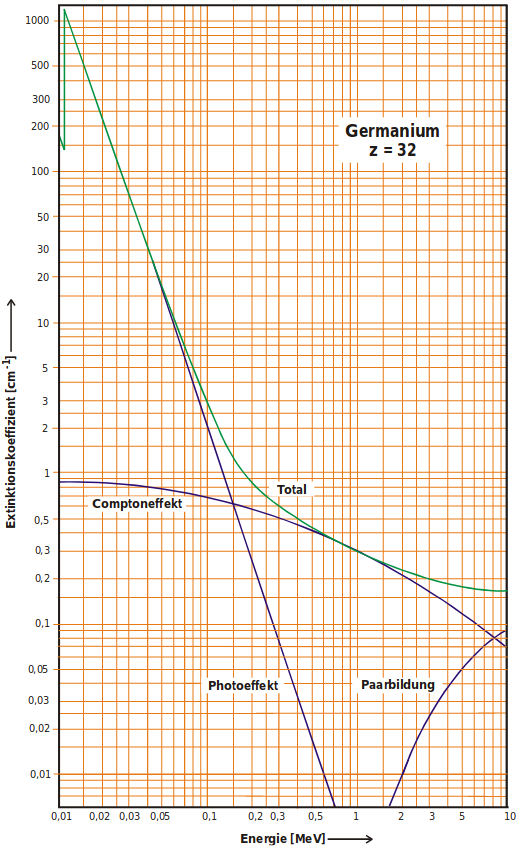
\includegraphics[width=0.9\textwidth]{Pics/crosssection.png}
  \caption{Extinktionskoeffizienten der verschiedenen Wechselwirkungen von $\gamma$-Quanten mit Germanium\cite{anleitung}.}
  \label{fig:crosssection}
\end{figure}

\subsection{Photoeffekt}
\label{subsec:photo}

Der Photoeffekt beschreibt die Wechselwirkung eines $\gamma$-Quants mit einem
Hüllenelektron der bestrahlten Materie.
Phänomenologisch kann der Photoeffekt über die folgende Gleichung erklärt werden.

\begin{equation}
  \label{eqn:photo}
  \gamma + \ce{Atom -> Atom^+} + e^-
\end{equation}

Somit beschreibt der Photoeffekt die Ionisation eines Atoms.
Das eingehende $\gamma$-Quant besitzt die Energie $E_{\gamma} > E\ua{B}$.
Dabei ist $E\ua{B}$ die Bindungsenergie des Elektrons an dem Atom.
Die Energiedifferenz zwischen $E_{\gamma}$ und $E\ua{B}$ trägt das Elektron in Form
von kinetischer Energie.
Das ausgelöste Elektron hinterlässt in dem Atom ein Loch, welhes durch ein Elektron
aus einer höheren Schale gefüllt wird. Die dabei frei werdende Energie
ist typischer Weise im Bereich der Röntgenstrahlung. In guter Näherung kann angenommen
werden, dass diese Röntgen-Quanten den Absorber nicht verlassen.
Das bedeutet bei dem Photoeffekt ist davon auszugehen, dass die vollständige
Energie des $\gamma$-Quants im Absorber verbleibt.

Der Wirkungsquerschnitt des Photoeffektes ist für den in dem Versuch auftretenden
Energieberich approximativ mit
\begin{equation}
  \label{eqn:crosssection_photo}
  \sigma\ua{Ph} \sim \frac{z^\alpha}{E^{\num{3,5}}}
\end{equation}
gegeben. $z$ entspricht der Kernladungszahl der wechselwirkenden Materie und $\alpha$
ist eine Exponent mit $4 < \alpha < 5$\cite{anleitung}.

\subsection{Compton-Streuung}
\label{subsec:compton}

Der Compton-Effekt beschreibt die Streuung von $\gamma$-Quanten an freien Elektronen
und wird durch folgende Gleichung beschrieben.

\begin{equation}
  \label{eqn:compton}
  \gamma + e^- \ce{->} \gamma '+ (e^-)'
\end{equation}

Gleichung~\eqref{eqn:compton} sagt aus, dass ein Energieübertrag zwischen dem
$\gamma$-Quant und dem Elektron $e^-$ stattfindet.
Der Prozess ist in Abbildung~\ref{fig:compton} schematisch illustriert.

\begin{figure}
  \centering
  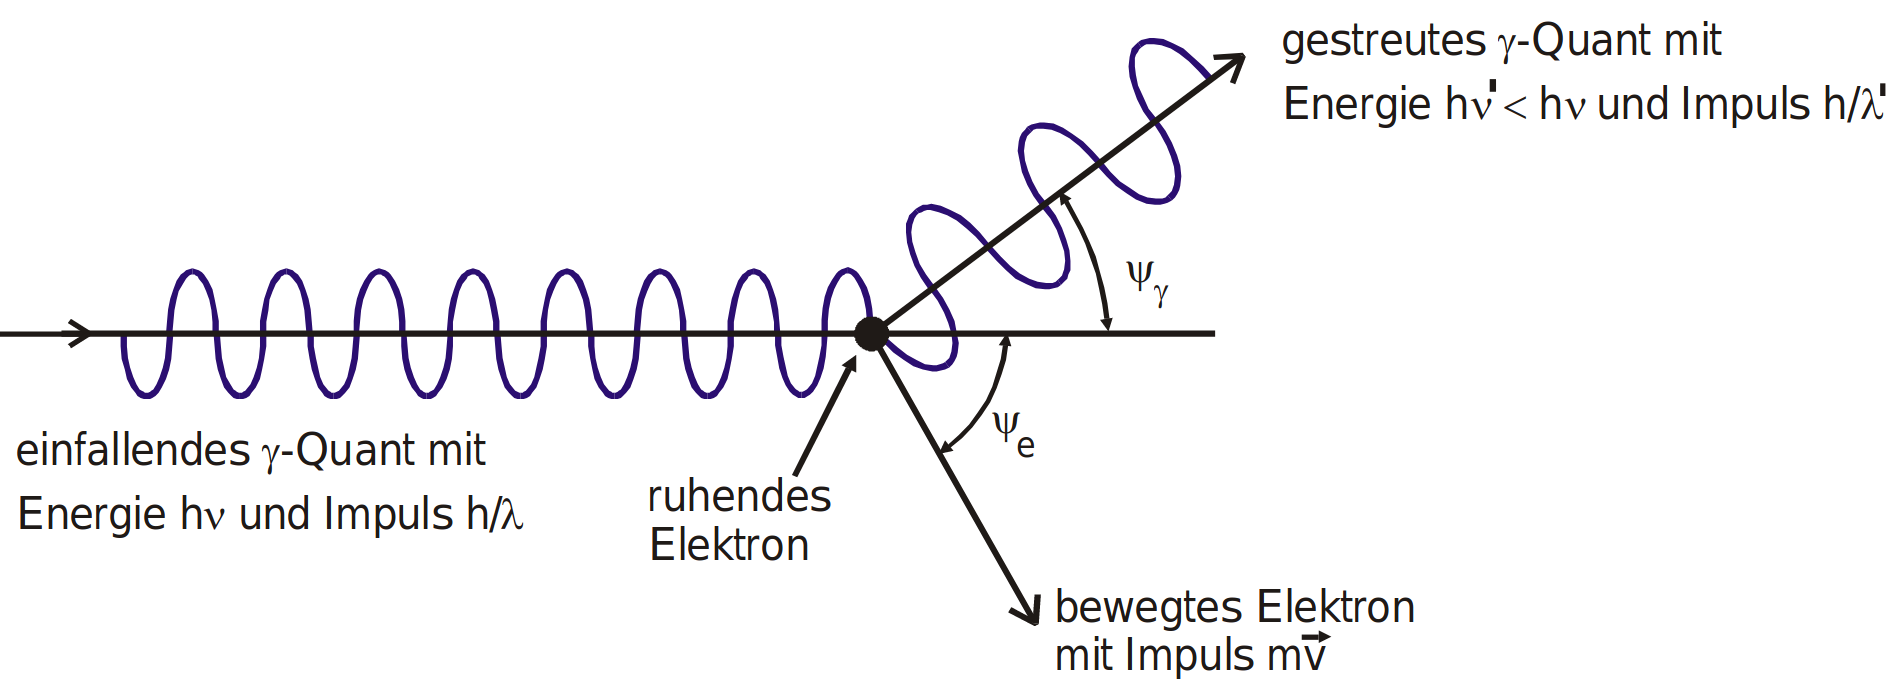
\includegraphics[width=0.9\textwidth]{Pics/compton.png}
  \caption{Schematische Darstellung der Compton-Streuung. $\Psi_\gamma$ ist der Streuwinkel des
  $\gamma$-Quants und $\Psi_{e^-}$ ist der Streuwinkel des gestoßenen Elektrons\cite{anleitung}.}
  \label{fig:compton}
\end{figure}

Die Impuls- und Energieerhlatung eines inelastischen Stoßen führen auf eine
$\gamma$-Quantenergie nach der Streuung $E_{\gamma}'$ von
\begin{equation}
  \label{eqn:comton_E_gamma}
  E_\gamma ' = E_\gamma\frac{m_0c^2}{m_0c^2 + E_\gamma\left(1 - \cos{(\Psi_\gamma)}\right)}.
\end{equation}
Die Energie des Elektrons nach der Streuung $E_{e^-}'$ ist gegeben durch
\begin{equation}
  \label{eqn:comton_E_el}
  E_{e^-}' = E-\gamma - E_\gamma ' = \frac{E_\gamma^2\left(1 - \cos{(\Psi_\gamma)}\right)}{m_0c^2 + E_\gamma\left(1 - \cos{(\Psi_\gamma)}\right)}.
\end{equation}
Der maximale Energieübertrag ist somit gegeben für $Psi_\gamma = \SI{180}{\degree}$,
was einer Rückstreuung entspricht. Der Bereich Streuung bei diesem Streuwinkel wird
im Energiespektrum als Compton-Kante bezeichnet (vgl. Kapitel~\ref{subsec:energiespektrum}).

\subsection{Paarbildung}
\label{subsec:paar}

Die Paarbildung tritt erst ab einer $\gamma$-Quantenergie von $E\gamma > 2m_0c^2$
auf, weshalb sie bei der hier betriebenen $\gamma$-Spektroskopie keinen
Einfluss hat. Der Prozess kann durch eine Gleichung der Form
\begin{equation}
  \label{eqn:paar}
  \gamma + \ce{Atom -> Atom} + e^+ + e^-
\end{equation}
erklärt werden. Aus Impulserhaltungsgründen ist die Energie des $\gamma$-Quants
auf beide Leptonen gleimäßig aufgeteilt.
Anstelle des Atoms in~\ref{eqn:paar} kann auch ein Elektron als Stoßpartner
fungieren, wobei die Paarbildung an Elektronen aufgrund einer höheren Schwellenenergie,
welche aus der geringeren Masse resultiert, unwahrscheinlicher ist.
Es wird nicht in jedem Fall die gesamte Energie eines einfallenden $\gamma$-Quants
im Absorber deponiert. Das erzeugte Positron rekonbiniert mit einem Elektron
des Absorbers, wobei aus Impulserhaltungsgründen zwei Photonen entstehen.
Mit einer endlichen Wahrscheinlichkeit kann eines der beiden, oder beide
Photonen nicht wieder mit dem Absorber wechselwirken und
den Detektor ohne Energiedeponierung verlassen.

\subsection{Wirkungsweise eines Reinst-Germanium-Detektors}
\label{subsec:wirkungsweise}
Germanium ist ein indirekter Halbleiter, weshalb ein Reinst-Germanium-Detektor
zu den Halbleiter-Detektoren gezählt wird.
Indirekte Halbleiter zeichnen sich dadurch aus, dass der geringste Abstand zwischen
Valenz- und Leitungsband
nicht direkt über dem $\su{\Gamma}$-Punkt liegt, sondern verschoben ist.
Aus diesem Grund wird für den Übergang eines Elektrons von dem Valenz-
in das Leitungsband noch ein zusätzliches Phonen benötigt, weshalb die
Anregungsenergie um ein Vielfaches größer ist als die eigentliche Bandlücke.

Halbleiter-Detektoren sind prinzipiell wie $pn$-Dioden aufgebaut.
$p$ und $n$ weisen auf die Dotierung des Halbleiters hin.
Bei $p$-dotierte Halbleiter werden Elektronen-Akzeptoren in den Halbleiter
eingebracht und bei $n$-dotierten Halbleitern werden Elektronen-Donatoren
eingebracht.
Im Bereich der Kontaktstelle zwischen $p$- und $n$-dotierten Halbleitern
entsteht eine Grenzschicht, in der die Donator-Elektronen mit den Akzeptor-Elektronen
rekombinieren. Diese Grenzschicht wird als Verarmungszone bezeichnet.
Die $p$-Schicht und die $n$-Schicht bilden aufgrund ihrer Unterschiedlichen
Dotierungen ein elektrostatisches Feld aus.
Auf die Verarmungszone einfallende $\gamma$-Quanten lösen durch die beschriebenen
Wechselwirkungsprozesse proportional zu ihrer Energie Elektronen aus.
Ein ausgelöstes Elektron hinterlässt eine positive Ladungslücke,
welche als Loch bezeichnet wird. Elektronen und Löcher diffundieren in dem
elektrostatischen Feld der $pn$-Diode zu den jeweiligen Elektronen und können dort
als Strom nachgewisen werden.

Außerhalb der Verarmungszone werden in einen Halbleiterdetektor die Elektronen
und Löcher nicht schnell genug getrennt, sodass diese rekombinieren und nicht
an den Elektronen nachgewiesen werden.
Aus diesem Grund ist es wichtig die Verarmungszone möglichst auszuweiten.
Das Ausweiten kann durch anlegen einer äußeren Spannung, der sogenannten Sperrspannung
$U$ bewirkt werden.
Bei Temperaturen ungleich Null entstehen sogenannte Leckströme, weshlab die Spannung
nicht beliebig groß sein kann. Leckströme entstehen beispielsweise durch Störstellen
oder durch das thermischen Auslösen von Elektronen in dem Detektormaterial.

Darüberhinaus kann die Verarmungszone durch eine extrem asymmetrische Dotierung
vergrößert werden, also zum Beispiel $n\ua{D}\gg n\ua{A}$.
In diesem Fall erstreckt sich die Verarmungszone über die gesamte $p$-Schicht.
\begin{figure}
  \centering
  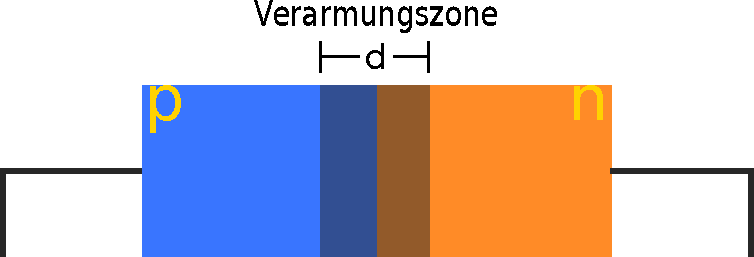
\includegraphics[width=0.8\textwidth]{Pics/pndiode.pdf}
  \caption{Schematische Abbildung einer $pn$-Diode mit einer Verarmungszone der Größe $d$.
  Das Anlegen einer Sperrspannung $U$ wird durch die eingezeichneten Elektroden angedeutet.}
  \label{fig:pndiode}
\end{figure}

\subsection{Energieauflösung eines Halbleiter-Detektors}
\label{subsec:energieauflösung}

Die Energieauflösung ist eine wesentliche Eigenschaft eines Detektors.
Sie kann anhand der Halbwertsbreite $\Delta E_{1 / 2}$ einer Impulshöhenverteilung
definiert werden. Qualitativ sagt dieses Kriterium aus, wie nah zwei
Mittelwerte von gleichen Gaußverteilungen zusammenliegen dürfe um noch
Eindeutig von einander unterscheidbar zu sein. Dieses Kriterium ist in
Abbildung~\ref{fig:energieauflösung} veranschaulicht.
Die Energieauflösung von indirekten Halbleiter-Detektoren wird von der statistischen
Verteilung der $\gamma$-Quantenergie auf die Phononen- und Elektronen-Loch-Paar-Erzeugung
beeinträchtigt.
Wird eine Poisson-Verteilung der Elektronen-Loch-Paar-Erzeugung angenommen
ergibt sich ein Fehler von
\begin{equation}
  \label{eqn:poisson}
  \sigma_{Poisson} = \sqrt{\bar{n}},
\end{equation}
mit $\bar{n}  = \frac{E_\gamma}{E\ua{E-L}}$.
Jedoch ist zu beachten, dass die Fluktioationen der Elektron-Loch-Paar-Erzeugung durch
Fluktuationen in der Phononenerzeugung teilweise kompensiert wird.
Diese Tatsache wird durch den Fano-Faktor $F < 1$ berücksichtigt.
Für Germanium wird ein Wert von $F\ua{Ge}\approx \num{0.1}$ angegeben\cite{anleitung}.\\
Ist die Anzahl der Elektronen-Loch-Paar-Erzeugungen sehr groß,
geht die Poisson-Verteilung in eine Gaußverteilung über, für die sich bei $E_\gamma = \SI{500}{\keV}$
eine Helbwertsbreite von
\begin{equation}
  \label{eqn:halbwertsbreite}
  \Delta E_{1/2}(\SI{500}{\keV}) \approx \SI{895}{\eV}
\end{equation}
ergibt.

Durch Leckströme~$H\ua{I}$, Feldinhomogenitäten in dem Detektor~$H\ua{E}$ und thermischen Rausches
in dem Detektor und der Ausleseelektronik~$H\ua{R}$
wird die Energieauflösung weiter beeinträchtigt.
Damit ergibt sich die Gesamthalbwertsbreite eines realen Detektors zu
\begin{equation}
  \label{eqn:reale_energieauflösung}
  H^2\ua{ges} = \Delta E_{1/2}^2 + H^2\ua{I} + H^2\ua{E} + H^2\ua{R} .
\end{equation}
Elektronisches Rausch und das Ausbliden von Leckströmen können durch Kühlen
des Detektors verringert werden. Die Feldinhomogenitäten des
elektrostatischen Feldes des Detektors kann durch Erhöhen der
Sperrspannung verringert werden, wobei sich die Leckströme antiproportional dazu
verhalten. Daher gibt es einen optimalen Bereich der Sperrspannung, indem
die addierte Halbwertsbreite beider Effekte minimal ist.

\begin{figure}
  \centering
  \includegraphics[width=0.8\textwidth]{Pics/energieauflösung.png}
  \caption{Veranschaulichung der Halbwertsbreite als qualifizierendes Merkmal der Energieauflösung eine Detektors.
  Dargestellt sind zwei Peaks monochromatischer $\gamma$-Strahler im Energiespektrum mit den
  Mittelwerten $E_1$ und $E_2$\cite{anleitung}.}
  \label{fig:energieauflösung}
\end{figure}

Neben der Energieauflösung werden Detektoren bezüglich ihrer Nachweiswahrscheinlichkeit
klassifiziert. Diese Nachweiswahrscheinlichkeit, oder auch Effizienz $Q$
beschreibt wieviele eingefallene $\gamma$-Quanten von dem Detektor
registriert werden.

\subsection{Energiespektren}
\label{subsec:energiespektrum}

Ein idealer Detektor würde beim Ausmessen einer monochromatischen Probe mit~$E_\gamma$
lediglich im Energiespektrum einen scharfen Peak an der Stelle $E_\gamma$
ausgeben. Ein realer Detektor produziert hingegen eine Energiespektrum der
Form von Abbilding~\ref{fig:spektrum}. Dieses entsteht, da der Compton-Effekt
keine diskrete, sondern eine streuwinkelabhängige kontinuierliche Energieverteilung
erzeugt, die von der Detektorakzeptanz bis zur Compton-Kante reicht.
Darüberhinaus entsteht ein Rückstreupeak aufgrund von größtenteils
außerhalb des Detektors rückgestreuten Photonen, welche mehrfach Compton-Streuung
machen.
Für die $\gamma$-Spektrometrie ist lediglich der Vollenergie-Peak
von bedeutung, da in diesem die gesamte Energie des $\gamma$-Quants
in dem Detektor deponiert wird. Bei $\gamma$-Quantenergie kleiner
als $\approx\SI{3}{\MeV}$ trägt lediglich der Photoeffekt zu dem relevanten
Vollenergie-Peak bei.

Wird eine nicht-monochromatische Probe betrachtet kann der Compton-Effekt
jedoch ebenfalls beiträge zu einem Vollenergie-Peak leisten.
Der Wirkungsquerschnitt des Compton-Effektes ist gemäß Abbildung~\ref{fig:crosssection}
für Energien von $E_\gamma>\SI{0.15}{\MeV}$ größer als der Wirkungsquerschnitt
der Photoeffektes, sodass es für diese Energien wahrscheinlicher ist, dass ein $\gamma$-Quant
Energie über Compton-Streuung deponiert. Wenn dieses $\gamma$-Quant
hinreichend viel Energie seiner anfänglichen Energie abgegeben hat,
wird der Photoeffekt wahrscheinlicher, sodass seine übrige Energie
vollständig in dem Detektor deponieren kann.
Aus diesem Grund wird der Peak nicht Photopeak, sonder Vollenergie-Peak genannt.

\begin{figure}
  \centering
  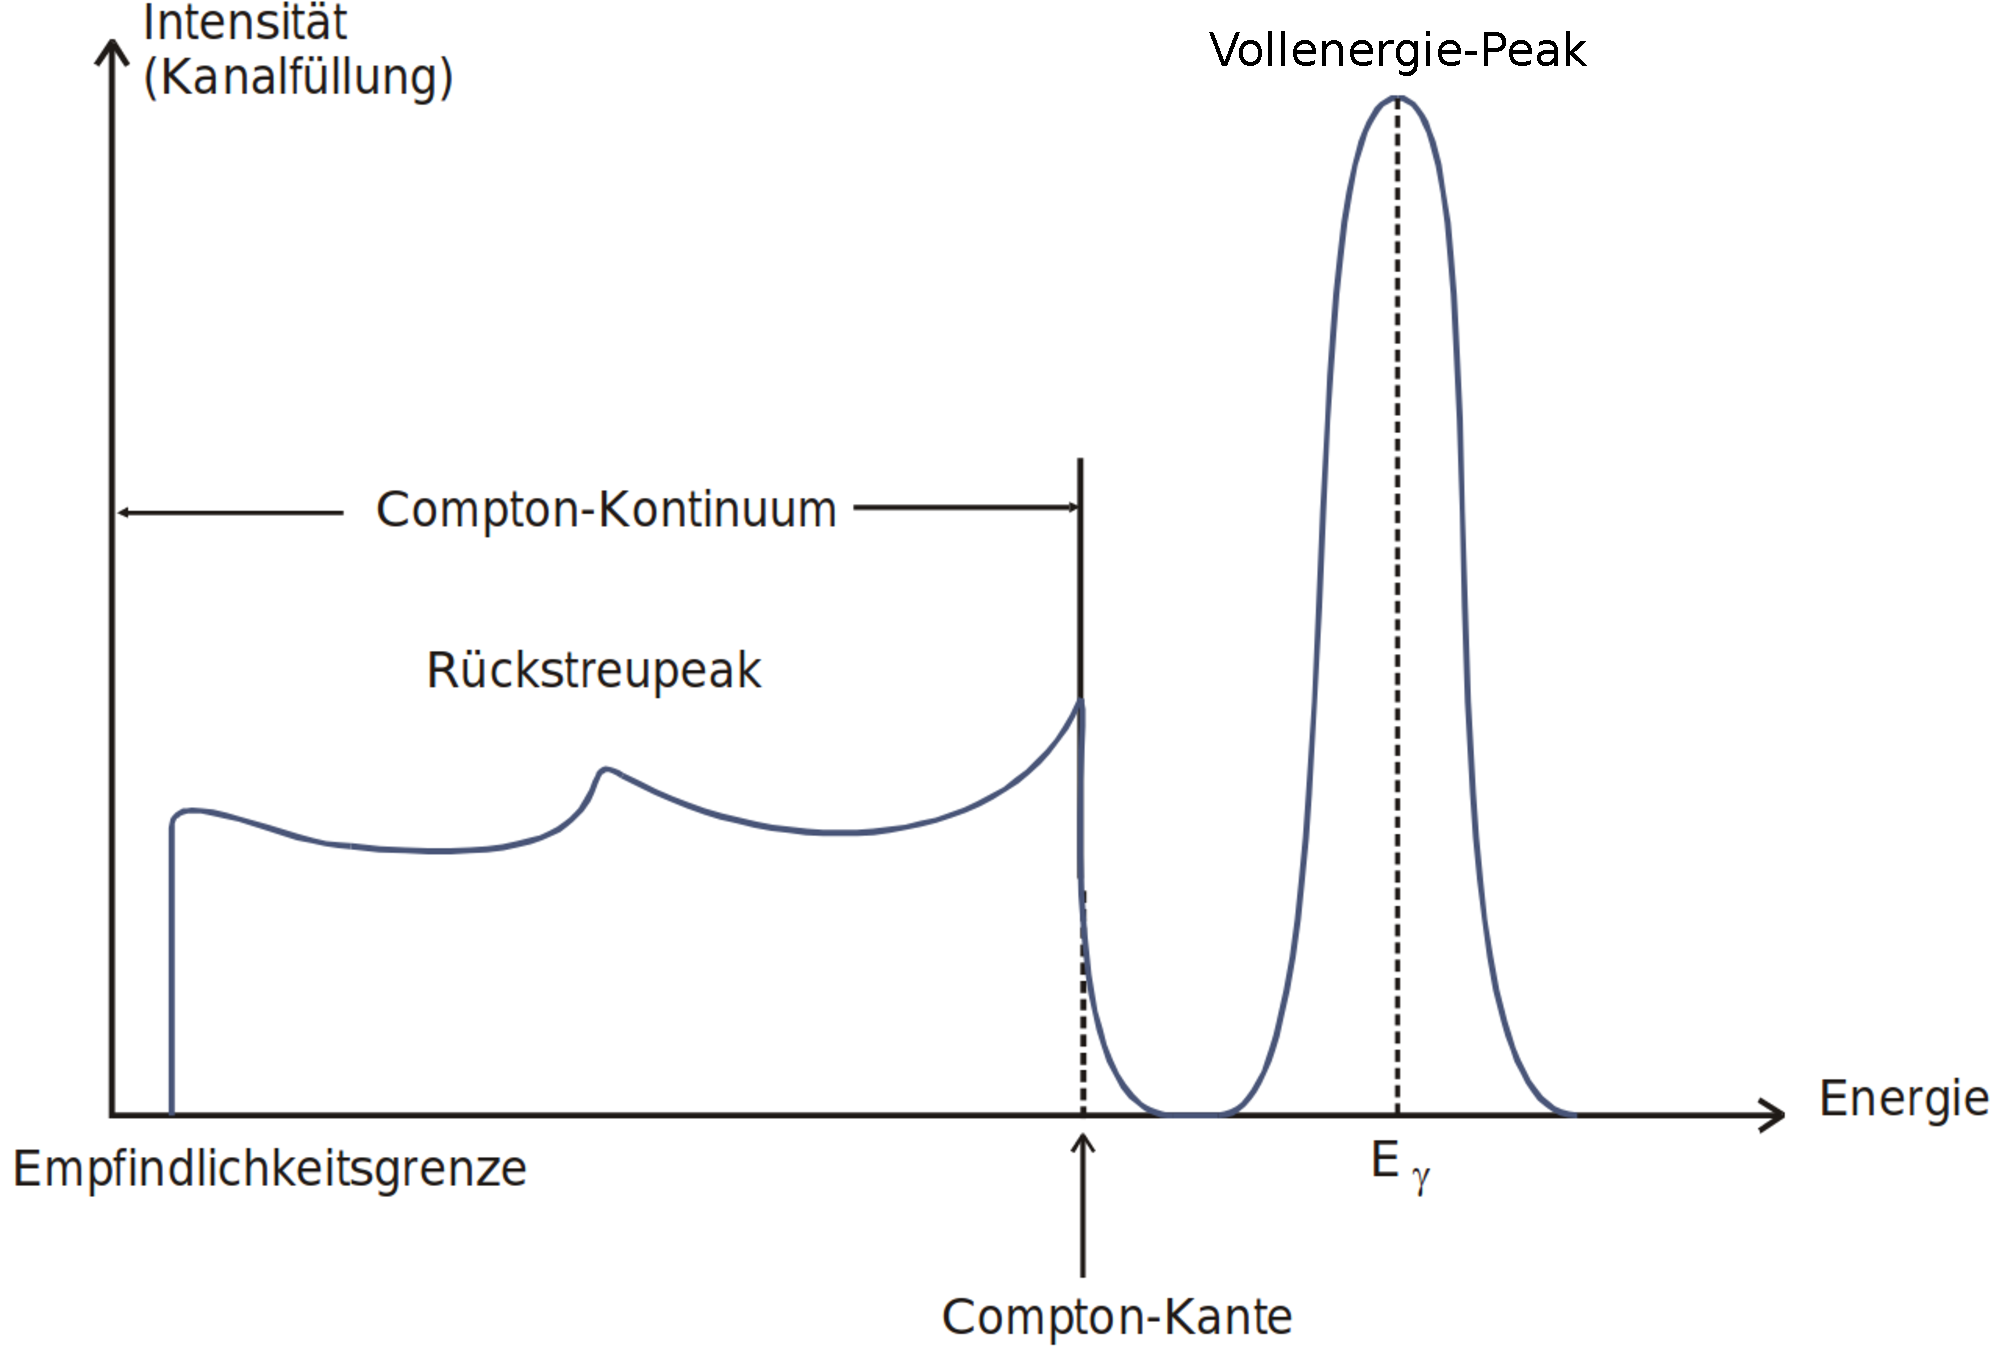
\includegraphics[width=0.8\textwidth]{Pics/spektrum.pdf}
  \caption{Gemessenens Energiespektrum einer monochromatischen Quelle (nach Quelle \cite{anleitung}).}
  \label{fig:spektrum}
\end{figure}

\section{Aufbau}
\label{sec:Aufbau}

\begin{figure}
  \centering
  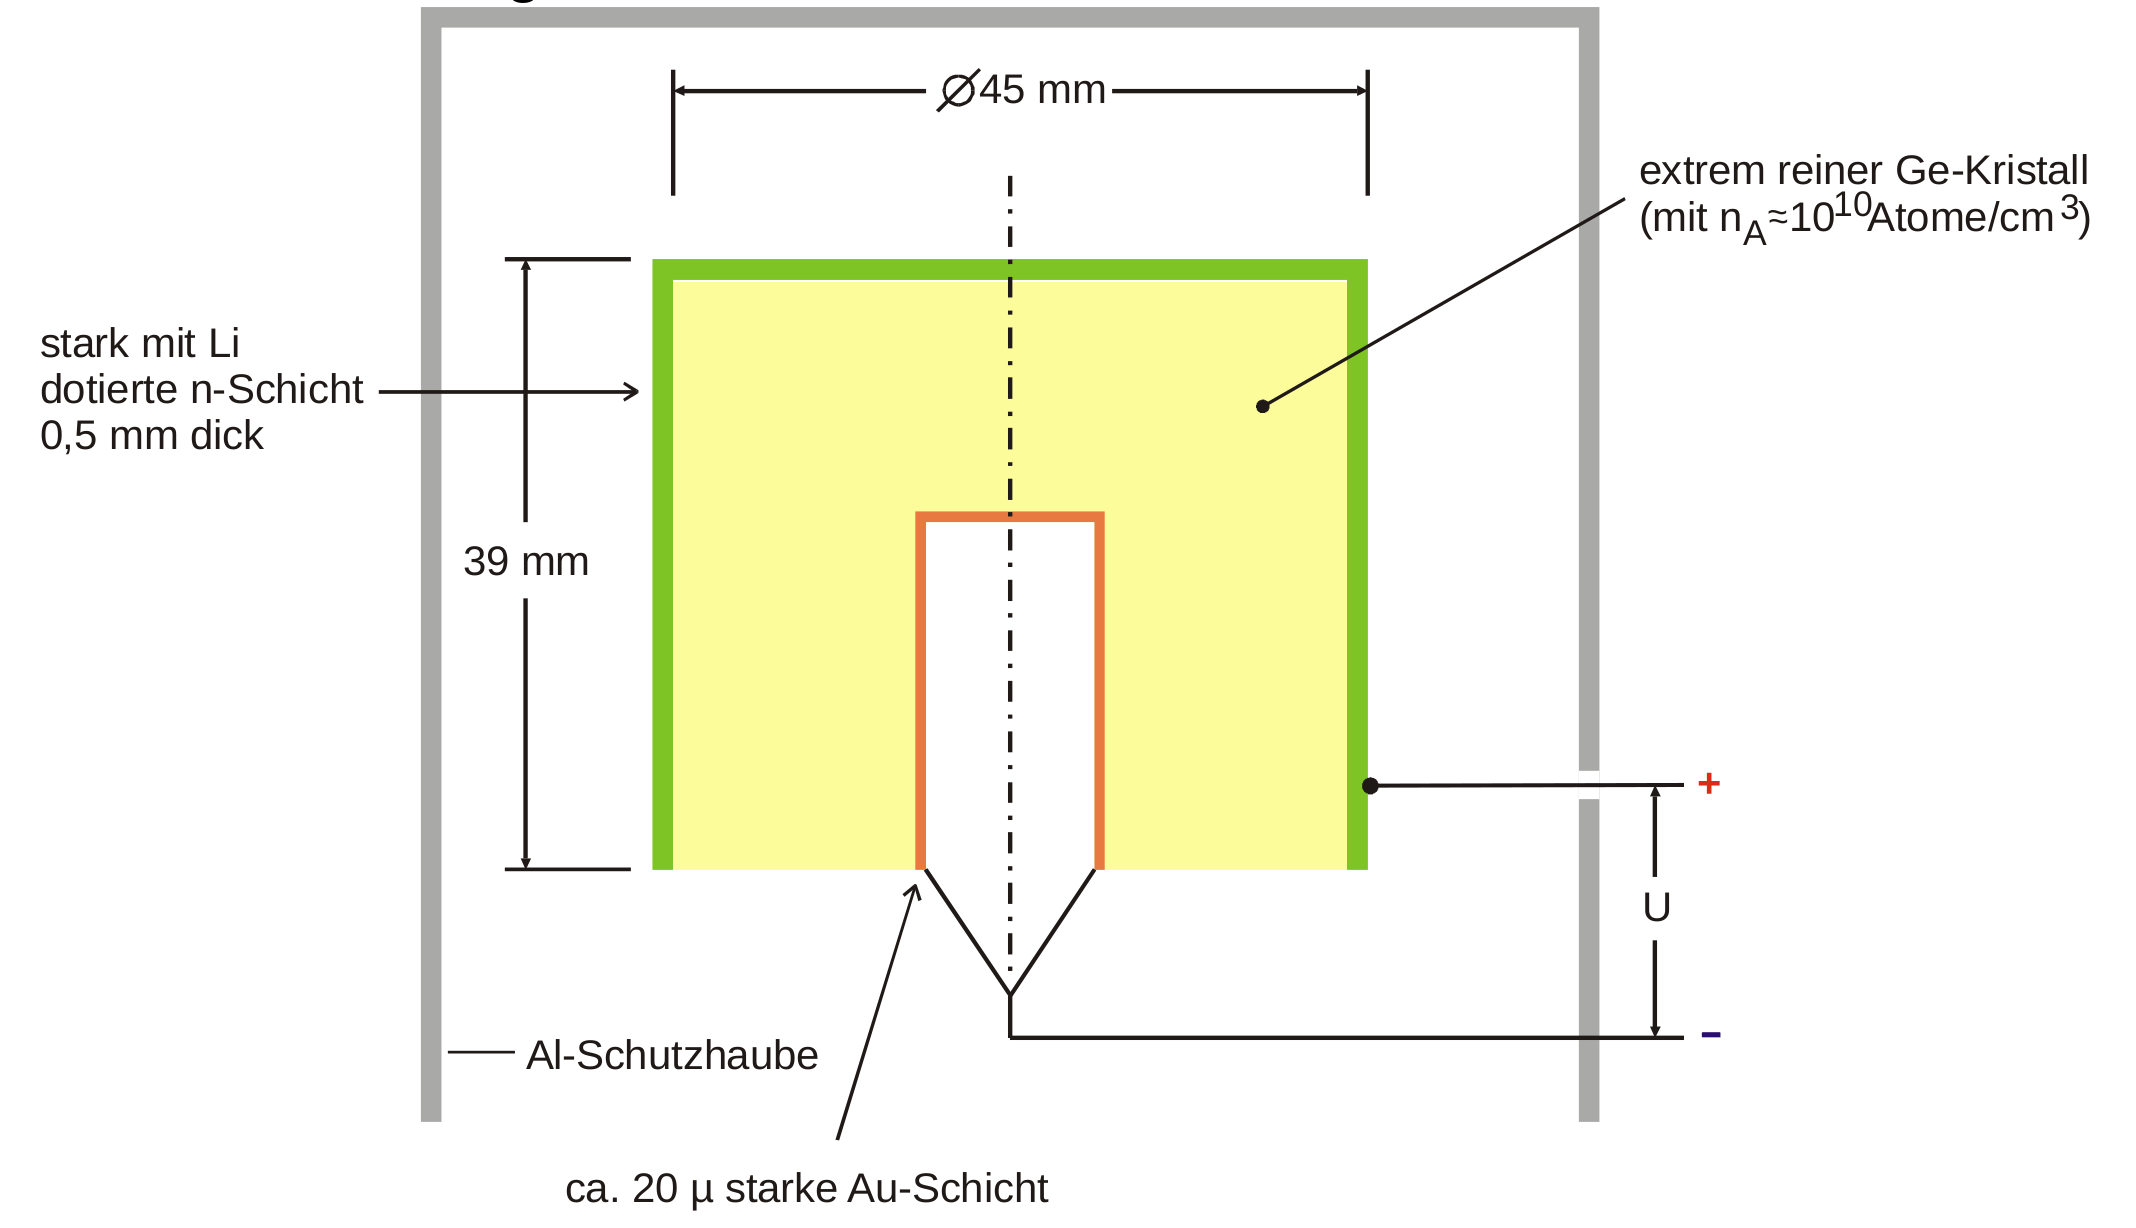
\includegraphics[width=0.85\textwidth]{Pics/aufbau.png}
  \caption{Schematischer Aufbau eines $\ce{Ge}$-Detektors. Nicht eingezeichnet sind
  die den gesamten Detektor umschließenden Abschirmungsschichten aus Kupfer und Blei\cite{anleitung}.}
  \label{fig:aufbau}
\end{figure}

\section{Durchführung}
\label{sec:durchführung}
